\documentclass[a4paper,12pt,article]{memoir}
%
% standard engelsk opsaetning
\usepackage[utf8]{inputenc}   % ʯÂ
\usepackage[english]{babel}            % engelsk opsÊtning
\usepackage{memhfixc}
\usepackage[T1]{fontenc}
\usepackage{lmodern} % lidt bedre CM font
%\usepackage{kpfonts}

% Matematiske symboler og fede tegn i ligninger
\usepackage{amsmath, amssymb, bm, bbm, dsfont, mathtools, mathdots, mathrsfs}


% Andet
\usepackage{fixltx2e} % retter noget
%\usepackage{hyperref} % g¯r at alle krydsreferencer, citeringer og indholdsfortegnelser bliver lavet om til interne hyperlinks.
\usepackage{afterpage}

% Henvisninger
\usepackage{url}
\usepackage{natbib} 
\citestyle{plain} % Plain Style citations
\makeatletter % Suppress various auxiliary commands in bib-file
\newcommand\Firstpublished[1]{\expandafter\ignorespaces\@gobble}
\newcommand\Editedby[1]{\expandafter\ignorespaces\@gobble}
\newcommand\biband{\expandafter\ignorespaces\@gobble}
\newcommand\Bookreview{\expandafter\ignorespaces\@gobble}
\newcommand\Moviereview{\expandafter\ignorespaces\@gobble}
\makeatother

% Tabeller og s¯jler
\usepackage{array, booktabs, dcolumn}
\newcolumntype{d}[1]{D{,}{,}{#1}} % Justering under komma

% Udvidelse til Matric Milj¯
\makeatletter
\renewcommand*\env@matrix[1][*\c@MaxMatrixCols c]{%
  \hskip -\arraycolsep
  \let\@ifnextchar\new@ifnextchar
  \array{#1}}
\makeatother

% Figurer og farver
\usepackage{graphicx, caption, subfig, xcolor}
\captionsetup{font=small,labelfont=bf}

% Saetninger
\usepackage{amsthm}
%\usepackage[standard,amsmath,amsthm]{ntheorem}

\theoremstyle{plain}
\newtheorem{thm}{Theorem}[section]
\newtheorem*{thm*}{Theorem} % uden nummer
\newtheorem{fthm}{Main Theorem}[section]
\newtheorem*{fthm*}{Main Theorem} % uden nummer
\newtheorem{lem}[thm]{Lemma}
\newtheorem*{lem*}{Lemma}
\newtheorem{pre}[thm]{Proposition}
\newtheorem*{pre*}{Proposition}
\newtheorem{cor}[thm]{Corollary}
\newtheorem*{cor*}{Corollary}
\newtheorem{con}[thm]{Conjecture}

% Definitioner
\theoremstyle{definition}
\newtheorem{defn}[thm]{Definition}
\newtheorem*{defn*}{Definition}

% Bemaerkninger og deslige
\theoremstyle{remark}
\newtheorem{ex}[thm]{Example}
\newtheorem*{ex*}{Example}
\newtheorem{rem}[thm]{Remark}
\newtheorem*{rem*}{Remark}

% Pagestyle simpel dokument
\makepagestyle{mysimplestyle} %Min pagestyle med sidetal
\copypagestyle{mysimplestyle}{empty}
\makeoddhead{mysimplestyle}{Kenneth Rasmussen}{\quad}{\today}
\makeheadrule{mysimplestyle}{\textwidth}{\normalrulethickness}
\makeoddfoot{mysimplestyle}{}{\thepage\ af \thelastpage}{} %KrÊver to oversÊttelser
%\pagestyle{mysimplestyle} % Aktiver Simple pagestyle

% Pagestyle st¯rre opgave
\makeevenfoot{companion}{}{\thepage}{}
\makeoddfoot{companion}{}{\thepage}{}
\makeevenfoot{ruled}{}{\thepage}{}
\makeoddfoot{ruled}{}{\thepage}{}
\makeevenfoot{plain}{}{\thepage}{}
\makeoddfoot{plain}{}{\thepage}{}
\pagestyle{ruled}

% lidt marginer
\setlrmarginsandblock{3cm}{*}{1}
\setulmarginsandblock{3cm}{*}{1}
\setheadfoot{2cm}{\footskip}          % mere h¯jde til header
\checkandfixthelayout[nearest]
\renewcommand{\baselinestretch}{1.3}

% Nummering-/inholdsfortegnelsesdybde
\setsecnumdepth{subsection}
\settocdepth{subsection}

% Punktopstilling
\usepackage{enumerate}

% Til specielle matricer
\usepackage{blkarray, gauss}

%\R for reelle tal og \C for komplekse og \N og de normale
\newcommand{\R}{\mathbb{R}}
\newcommand{\C}{\mathbb{C}}
\newcommand{\N}{\mathbb{N}}
\newcommand{\Z}{\mathbb{Z}}
\newcommand{\Q}{\mathbb{Q}}
\newcommand{\K}{\mathbb{K}}
\renewcommand{\P}{\mathbb{P}}
\newcommand{\D}{\mathbb D}
\newcommand{\F}{\mathbb{F}}
\newcommand{\infi}{\mathcal{O}} %point at infinity

% Kommandoer specielt til p-adiske tal
\newcommand{\p}[1]{\left\lvert #1 \right\rvert _p} % p-adisk absolut vÊrdi
\newcommand{\pp}[1]{\left\lVert #1 \right\rVert _p} % p-adisk absolut vÊrdi 2 streger

% Kommandoer
\newcommand{\abs}[1]{\left\lvert #1 \right\rvert} % absolut vÊrdi
\newcommand{\pdiff}[2]{\frac{\partial #1}{\partial #2}}

%partielle differentialer
\DeclareMathOperator*{\maks}{maks} 
\newcommand{\aut}{\mathrm{Aut}}

% Ekstra kommandoer Mads
\newcommand{\iprod}[2]{\langle #1 , #2\rangle}
\newcommand{\spor}[1]{\textrm{tr}( #1 )}
\newcommand{\dnorm}[1]{\Vert #1 \Vert}
\newcommand{\enorm}[1]{\left\lvert #1 \right\rvert}
\newcommand{\sset}[1]{\lbrace #1 \rbrace}
\newcommand{\Sset}[1]{\left\{ #1 \right\}}
\newcommand{\msum}{\sum_{\alpha \in \mathbb N_0^n}} 

\theoremstyle{plain}
\newtheorem{lemma}[thm]{Lemma}

\theoremstyle{remark}
\newtheorem*{bemrk}{Remark}

\usepackage[draft,english]{fixme} %in text: \fxnote{..}
\fxsetup{layout=footnote,marginclue}


% Citater
\newsavebox{\citeret}
\newenvironment{citat}[1]{%
  \sbox{\citeret}{--- \textsf{#1}}%
  \begin{flushright}\itshape}%
  {\par \usebox{\citeret}\end{flushright}}

%Functions
\newcommand{\Char}{\text{char}}
\newcommand{\probi}{\text{prob}}

%Algorithms
\usepackage[section]{algorithm}
\usepackage{algpseudocode}
\renewcommand{\algorithmicrequire}{\textbf{Input:}}
\renewcommand{\algorithmicensure}{\textbf{Output:}}
\algnotext{EndFor}
\algnotext{EndIf}
\algnotext{EndWhile}


 \makepagestyle{aflevering}
 \makeevenfoot{aflevering}{}{\thepage}{}
 \makeoddfoot{aflevering}{}{\thepage}{}
 \makeoddhead{aflevering}%
 	{Torben Hansen, F120116 \\ Parallel Algorithms Mastermath fall 2012}%
 	{}%
 	{Project 2}
 \pagestyle{aflevering}
 % Forfatter og titel
\title{\textbf{Parallel Sorting }}
\author{Torben Hansen, F120116}
\date{Utrecht University - Institute of Mathematics}

\renewcommand{\labelitemi}{$-$}
\usepackage{titlesec}
\titleformat{\section}{\large\bfseries}{\thesection}{1em}{}
%  
\begin{document}
%
\maketitle
ffffddThis project aims to develop a parallel sorting algorithm. The algorithm developed is a merging like parallel sorting algorithm with BSP complexity
\begin{align*}
O\left((2\log_2(p)+1)l+\frac{n}{p}\log_2\left(\frac{n}{p}\right)+(p-1)\frac{n}{p}+g(p-1)\frac{n}{p}\right).
\end{align*}
This complexity is far from optimal compared to other parallel sorting algorithms in the literature. 

It is also clear from the experiments in chapter 3 that this algorithm performs poorly compared to other sorting algorithms and has a very bad scaling. 

\newpage
\begin{tableofcontents}*
\end{tableofcontents}
\newpage

\chapter{Sequential sorting \textit{merge sort}}
In this chapter we will present a sequential sorting algorithm called merge sort. This is a well known algorithm that uses a divide-and-conquer approach. That is, recursively splitting the sequence to be sorted into smaller pieces and thereafter merge all the pieces together again in a recursive manner. 

\section{The sorting problem}
In general sorting you do not necessarily restrict to sorting numbers. It can be any kind of set of objects on which a partial ordering can be established. Hence the general problem is: Given a sequence of objects $\langle a_1,a_2,\ldots,a_n\rangle$, find a permutation $\sigma\in S_n$ such that $a_{\sigma(1)}\leq a_{\sigma(2)}\leq \cdots \leq a_{\sigma(n)}$ and output the sequence $\langle a_{\sigma(1)},a_{\sigma(2)},\ldots,a_{\sigma(n)}\rangle$. Here the operator $\leq$ defines the partial ordering. The algorithm developed in this paper is capable of solving the general sorting problem. In general, not every sorting algorithm can do this e.g. Radix sort or counting sort. 

We assume in the rest of this paper that checking whether $a \leq b$ takes constant time. 

\section{The algorithm}
Explicitly writing down the divide-and-conquer behaviour of merge sort makes the algorithm easy to write down: Say we have $n$ elements to sort then

\textbf{Divide} Divide the $n$ elements sequence to be sorted into two subsequences of $n/2$ elements. 

\textbf{Conquer} Sort the two subsequences recursively using merge sort. 

\textbf{Combine} Merge the two sorted sequences to produce the sorted answer.  
\\
That is, we need two algorithms: a merge algorithm and an algorithm that is called recursively. Algorithms \ref{alg:merge} and \ref{alg:mergeSort} constitute the merge sort algorithm. 

Note that we give algorithms that are easy to analyse and therefore the implementation of these algorithms in \textit{bspParSort} differs a bit. 

To start the algorithm the initial call is Merge-sort($A$,$0$,$n-1$).

\begin{algorithm}
\caption{Merge}
\label{alg:merge}
\begin{algorithmic}[1]
\Require Array $A$. Assume we wish to merge $A[l..m]$ and $A[m+1..r]$ and assume that the two sub arrays are sorted. 
\Ensure For all $i,j$ with $l\leq i\leq j\leq r$ we have $A[i]\leq A[j]$. 
\State Create array $L$ with $\vert L\vert =m-l+1$ containing elements $A[l..m]$ in place. Similarly create $R$ with $\vert R\vert=r-m$ containing $A[m+1..r]$ in place. 
\State Set $L[(m-l+1)+1]=\infty$ and $R[(r-m)+1]=\infty$
\State $i=j=0$
\For{$k=l \to r$}
\If{$L[i]\leq R[j]$}
\State $A[k]=L[i]$
\State $i=i+1$
\Else 
\State $A[k]=R[j]$
\State $j=j+1$
\EndIf
\EndFor
\end{algorithmic}
\end{algorithm}

\begin{algorithm}
\caption{Merge-sort}
\label{alg:mergeSort}
\begin{algorithmic}[1]
\Require Array $A$ containing $n$ elements and indices $l,r$. 
\Ensure Sorted sub array $A[l..r]$. 
\If{$l<r$}
\State $m=\left\lfloor \frac{r+l}{2}\right\rfloor$
\State Merge-sort($A$,$l$,$m$)
\State Merge-sort($A$,$m+1$,$r$)
\State Merge($A$,$l$,$m$,$r$)
\EndIf
\end{algorithmic}
\end{algorithm}
\section{Complexity}
We may assume WLOG that $n=2^k$ for some $k$. Clearly, algorithm \ref{alg:merge} takes no more than $O(n)$ time. Let $T_{mergeSort}$ denote the time to run algorithm \ref{alg:mergeSort}, with $T_{mergeSort}(1)=O(1)$. Then we get the recurrence $T_{mergeSort}(n)=2T_{mergeSort}(n)+cn$. By induction it is easily proven that $T_{mergeSort}(n)=2^mT_{mergeSort}(n/2^m)+mcn$. Since we in every round split the sequence of numbers in half, we terminate when $m=k=\log_2(n)$. Hence $T_{mergeSort}(n)=nT_{mergeSort}(1)+cn\log_2(n)=O(nlog_2(n))$. Since every comparison based sorting algorithm satisfy the lower bound $\Omega(n\log_2(n))$ we have $T_{mergeSort}(n)=\Theta(n\log_2(n))$. 
\newpage

\chapter{Parallel sorting \textit{bspParSort}}
In this chapter we present the parallel sorting algorithm. The algorithm presented could be considered a parallel merge sort. 

In our situation, we say that it is only necessary for processor 0 to know about the result - in a situation in which the result should be known by everyone, a broadcast in the end could be added. In addition we assume that we are sorting integers but the algorithm could be extended to solve the general sorting problem. We also assume that the number of processors $p$ is a power of 2 and that $n$ is divisible by $p$. In math this is $p=2^k$ for some non-negative $k$ and $p\vert n$. 
  
\section{Idea}
The main idea of the algorithm builds on the idea the merge sort but with some extra work to before the merging and a more complicated merging. The way we take advance of the availability of more processors than one, is to first distribute disjoint parts of the sequence of numbers to each processor and such that we get all the sequence distributed. Thereafter perform a local sort on each of the sub sequences on each processor using a sequential sorting algorithm (in our case merge sort). The problem now is to cook up a scheme of merging that, in the end, gives the sorted sequence at processors 0. 

\section{Distribution and communication}
\textbf{Distribution} Say we want to partition the array $A[0..n-1]$ with $A[i]$ an integer using $p$ processors $P(0),P(1),\ldots,P(n-1)$. As we are going to do a local sort, we strive to obtain the most evenly distribution as possible. Since we assume that $p$ divides $n$ this is easily obtained by a block distribution. That is, each processor contains $n/p$ elements with processor 0 containing $A[0..n/p]$, processor 1 containing $A[(n/p)+1..2n/p]$, etc. 

If a priori we knew more about the sequence of numbers, it would indeed be possible to make a better distribution. But taking into account the possibility of completely random sequences and the use of a local sort, this distribution must be considered a good choice. 

\noindent\textbf{Communication} Let $s$ be a particular processor. After the local sort a series of communications are required to merge the sub sequences into a final sorted sequence on processor 0. The scheme we have fixed on does this in a uni directional way by recursively merging one half of the sub sequences into another unique half. The local merging is similar to the merging done in merge sort.  

As an example, consider this scheme in a situation with 4 processors and the point right after the local sort. Then we send the sequence from processor 2 and 3 to processor 0 and 1 respectively and perform a local merge on processor 0 and 1. After that we have reduced the number of ``active'' processors to half the original amount. In the next merging round we send the new sequence on processor 1 to processor 0 and perform a local merge on processor 0. The results is the original sequence but now sorted. 

With the idea in hand we now dig further into how the merging and communication is done. The problems that arise are the following: which processors are going to receive, send or be idle (not used any more) in a particular round and which processors should be matched. Say we are in round $j$ of the merging scheme. In each round we have halved the number of active processors and are therefore left with $p/2^{j-1}$ active processors which means that all processors satisfying $s\geq p/2^{j-1}$ are idle. Of those processors that are not idle the first half should receive and the other half send, i.e. if $s<p/2^j$ processor $s$ should receive. The processor that $s$ should receive from is easily determined as processor $s+p/2^j$. 

Notice that all of this only work because we assume $p$ is a power of 2. 
\section{Description and pseudo code}
In this section we present pseudo code for the parallel algorithm. The full implementation can be read in appendix A. Algorithm \ref{alg:parSort} contains the pseudo code. We add additional comments to the pseudo code below
\begin{itemize}
\item In the pseudo code no print-out-statement of the final result is added. This is trivial for the user to implement by himself and wont change the asymptotic behaviour of the algorithm.
\item The merging between $A_s$ and $temp$ in line 10 is done in a similar fashion as in algorithm \ref{alg:merge}. In round $j$ the number of elements to be merged is $2^{j-1}(n/p)$. 
\item The C-implementation also contains a parse section that reads a text document containing the sequence of numbers to be sorted, writes these numbers into an array on processor 0 and thereafter sets up the distribution.  
\end{itemize}
\begin{algorithm}
\caption{bspParSort}
\label{alg:parSort}
\begin{algorithmic}[1]
\Require The number of processors $p$. Using the distribution described in section 2.2. We let $A_s$ denote the local array with $\vert A_s\vert = n/2^{\lceil \log_2(s+1)\rceil}$. We assume $A_s$ has been pushed to the stack. 
\Ensure The original sequence sorted. Located in $A_0$. 
\State (0)
\State mergeSort($A_s$,$0$,$(n/p)-1$) 
\For{$j=1\to \log_2(p)$}
\State (1)
\If{$s<p/2^j$}
\For{$k=0\to 2^{j-1}(n/p)-1$}
\State get $A_s[k]$ from $P(s+p/2^j)$ (Assume $A_s[0..2^{j-1}(n/p)-1]$ goes to an array $temp$)
\EndFor
\EndIf
\State (2)
\If{$s<p/2^j$}
\State Merge $A_s$ and $temp$
\EndIf
\EndFor
\end{algorithmic}
\end{algorithm}

\section{BSP cost}
To do the analysis we assume that it take $O(n\log_2(n))$ flops to sort $n$ elements using merge sort. Clearly we can analyse the BSP cost by looking only at processor 0. 

By the assumption above superstep 0, which is a computational superstep, cost $\delta (n/p)\log_2((n/p))+l$ flops for some constant $\delta$. This constant factor very much depends on the sequence of numbers being sorted. 

Superstep 1 is a communication superstep that transfers elements from one half of the (non-idle) processors to the others. In round $j$ processors with $s<p/2^j$ gets $2^{j-1}(n/p)$ data words from processor $s+p/2^j$ i.e. this step costs $g2^{j-1}(n/p)+l$.

Superstep 2 is a computational superstep that merges two arrays. In round $j$ each array contains $2^{j-1}(n/p)$, so merging takes $\mu 2^{j-1}(n/p)$ flops for some (small) constant $\mu$. Hence this step costs $\mu 2^{j-1}(n/p)+l$

Table 1 sums up the cost of each superstep. Let $T_{bspParSort}$ denote the BSP cost of $bspParSort$. Since the for-loop starting in line 3 takes $\log_2(p)$ step we have
\begin{align*}
T_{bspParSort}&=\delta \frac{n}{p}\log_2\left(\frac{n}{p}\right)+l+\sum_{i=1}^{\log_2(p)}(g2^{i-1}\frac{n}{p}+l)+\sum_{j=1}^{\log_2(p)}(\mu 2^{j-1}\frac{n}{p}+l) \\
&=2\log_2(p)l+l+\delta \frac{n}{p}\log_2\left(\frac{n}{p}\right)+\mu\frac{n}{p}\sum_{j=1}^{\log_2(p)} 2^{j-1}+g\frac{n}{p}\sum_{i=1}^{\log_2(p)}2^{i-1} \\
&=(2\log_2(p)+1)l+\delta\frac{n}{p}\log_2\left(\frac{n}{p}\right)+\mu(2^{\log_2(p)}-1)\frac{n}{p}+g(2^{\log_2(p)}-1)\frac{n}{p} \\
&=(2\log_2(p)+1)l+\delta\frac{n}{p}\log_2\left(\frac{n}{p}\right)+\mu(p-1)\frac{n}{p}+g(p-1)\frac{n}{p}
\end{align*}
In addition to the BSP cost, one can add that the algorithm uses $O(n)$ of extra space on each processor. 

The BSP cost analysis shows a rather poor scaling of $bspParSort$. Indeed we can write $\mu(p-1)\frac{n}{p}+g(p-1)\frac{n}{p}$ as $\mu(n-n/p)+g(n-n/p)$, which shows that increasing the number of processors would have a negative effect on these two terms. 
\begin{table}
\begin{center}
\begin{tabular}{|c|c|}
\hline 
\#Superstep & Cost \\ 
\hline 
0 & $\delta n\log_2(n)+l$ \\ 
\hline 
1 & $g2^{j-1}(n/p)+l$ \\ 
\hline 
2 & $\mu 2^{j-1}(n/p)+l$ \\ 
\hline  
\end{tabular} 
\caption{BSP cost for algorithm \ref{alg:parSort}}
\end{center}
\end{table}
\newpage

\chapter{Experiments}
In this chapter we test our implementation of \textit{bspParSort} discussed in the last chapter. Our strategy is first to benchmark the computer we are using and then compare empirical data with the expected theoretical performance. We will be testing the implementation on the supercomputer \textit{Huygens}. 
\section{Benchmark}
To do the benchmark we use the already implemented version from the \textit{BSPedupack} but with $bsp\_put$ replaced with $bsp\_get$. 
\begin{table}
\label{table:benchgetHuygens}
\begin{center}
\begin{tabular}{|c|c|c|c|}
\hline 
$p$ & $r$ (Mflop/s) & $g$ & $l$ \\ 
\hline 
1 & 169.110 & 73.6 & 566.1 \\ 
\hline 
2 & 182.821 & 81.5 & 2577.9 \\ 
\hline
4 & 195.121 & 90.5 & 6731.8 \\
\hline
8 & 195.375 & 98.8 & 13428.3 \\
\hline
16 & 192.975 & 98.3 & 26778.5\\
\hline
\end{tabular}
\caption{Benchmark \textit{Huygens} with $bsp\_ get$.}
\end{center}
\end{table}

\section{Results}
Here we present our results. Experiments have been done with the following method: we consider an integer $2^b$ for a $b$ between 10 and 20. With this number we generate a sample set of $2^b$ integers between $\approx -2300000000$ and $\approx 2300000000$ picked uniformly at random. With this sample set we measure the execution time for $p=1,2,4,8,16$ at $Huygens$. The results are displayed in the graphs below. We have divided the result into several plots to give a better view and comparison basis. As BSP library we have used BSPonMPI. 

A more serious study would have involved picking more sample sets ( depending on the variance of the results), and taking the average over a run with numbers in the sample space. Also a more universal study would have involved calculating the number of flops and a comparison with the result to the expected number of flops. In addition, one could also compute the utilization of the CPU with respect to flop/s. 
\begin{figure}[hbtp]
\centering
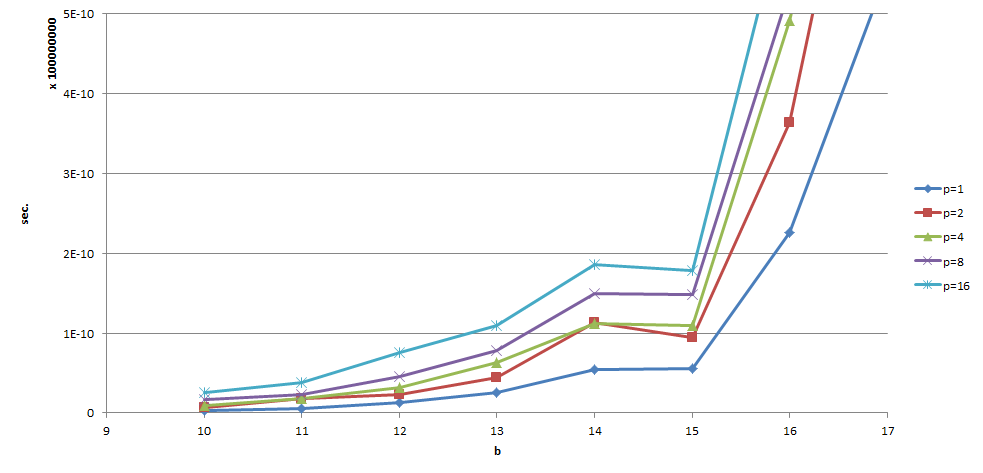
\includegraphics[scale=0.65]{exp1.png}
\caption{Clearly there is no advantage of using more processors.}
\end{figure}

\begin{figure}[hbtp]
\centering
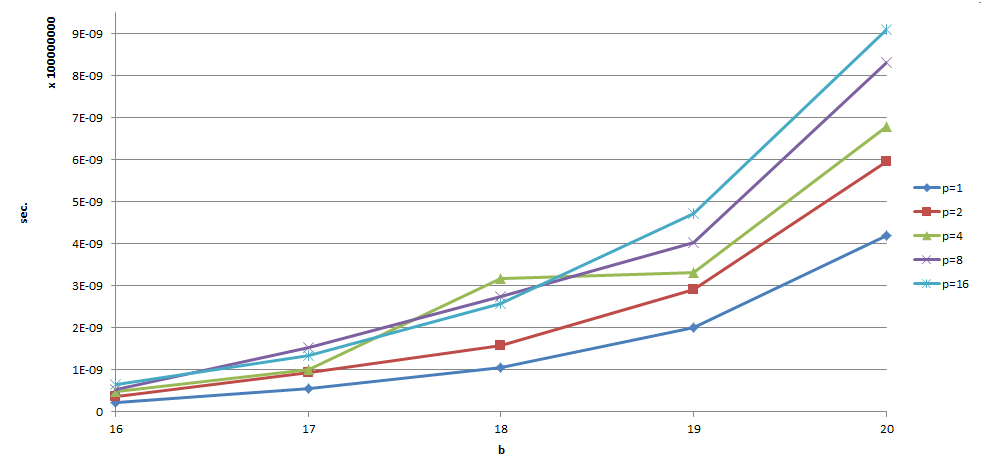
\includegraphics[scale=0.65]{exp2.png}
\caption{Signs of a larger and larger bias between the curves becomes more visible.}
\end{figure}

We have also calculated the theoretical time of $bspParSort$ for $p=4$. This is displayed in table 3. We have used the following formula to calculate the theoretical time 
\begin{align*}
&\frac{1}{r}\left((2\log_2(p)+1)l+\delta\frac{n}{p}\log_2\left(\frac{n}{p}\right)+\mu(p-1)\frac{n}{p}+g(p-1)\frac{n}{p}\right)\quad \mbox{with} \\
&\delta=2,\quad \mu=2,\quad p=4, \quad n=2^b,\quad g=90.5,\quad r=195.121,\quad l=6731.8.
\end{align*}

\begin{table}
\label{table:benchgetHuygens}
\begin{center}
\begin{tabular}{|c|c|c|c|}
\hline 
$b$ & sec. \\ 
\hline 
10 &  557.557 \\ 
\hline 
11 &  947.899 \\ 
\hline
12 &  1733.791 \\
\hline
13 &  3316.071 \\
\hline
14 &  6501.622\\
\hline
15 &  12914.709\\ 
\hline 
16 &  25824.852 \\ 
\hline 
17 &  51813.075 \\ 
\hline
18 &  104125.394 \\
\hline
19 &  209421.779 \\
\hline
20 &  421358.044\\
\hline
\end{tabular}
\caption{Theoretical time for $bspParSort$ with $p=4$}
\end{center}
\end{table}

\section{Comments}
A direct transformation of the merge sort algorithm into parallel doesn't give any speed-up at all. Actually, the experiments above show that increasing the number of processors has a direct negative effect on the running time. 

Observing figure 2, it is obvious that for bigger bit sizes the performance when increasing the number of processors becomes worse. 

Two issues that are likely to cause this bad performance are first of all the many idle processors, which are just non-used CPU power. Second in the end of the merging a large number of data words is moved between processors. 

Looking at table 3 one concludes that it does not even make sense to try to compare the theoretical time with the time measured in practice. But one can carefully conclude that the algorithm is far better in practice than in theory....

\appendix

\chapter{Parallel algorithm \textit{bspParSort}}
\begin{verbatim}
#include "bspedupack.h"
//#include "include/mcbsp.h"


/*
  This program sort an array of integers. 
  Invariants: P is a power of two and n is divisible by p.
  Notes: 
    - Data are distributed by the block distribution 
      (processor s contains n/p numbers). 
    - Not many boundary checks are performed. 
    - Merging is performed in a unidirected form (to the left). 
    - The text file storing the sequence must have the following format:
      [number of elements] [number 1] [number 2] etc
      And the file name must be named 'sort'.
*/


//Global fields
int P; /* number of processors requested */

void bspParSort(){

  int Log2(int x);
  void mergeSort(int x, int *temp1);
  void merge2(int *arr1, int *arr2, int size);

  int *localArr; /* local array in each processor */
  int i,j,k; /* index variables */
  int n_divide_p; /* Avoid multiple computation */
  int n; /* Number of elements to be sorted */
  int szLocalArray; /* Size of local array */
  double time0, time1; /* Time */
  FILE *ifp = 0; /* Reader to read sequence of numbers to be sorted */

  bsp_begin(P);
  int p= bsp_nprocs(); /* Number of processors obtained */ 
  int s= bsp_pid();    /* Processor number */ 

  //Get number of elements to be sorted
  if(s==0){
    ifp = fopen("sort","r");
    if(ifp == NULL){
      fprintf(stderr, "Can't open input file!\n");
      exit(1);
    }
    fscanf(ifp, "%i", &n);
  }

  // Make sure every processor knows everything
  bsp_push_reg(&n,sizeof(int));
  bsp_sync();
  bsp_get(0,&n,0,&n,sizeof(int));
  bsp_sync();
  bsp_pop_reg(&n);

  //Setup distribution 
  n_divide_p = n/p;
  szLocalArray = n/pow(2,ceil(Log2(s+1)));
  localArr = vecalloci(szLocalArray);
  bsp_push_reg(localArr,sizeof(int)*szLocalArray);

  if(s==0){ 
    printf("Distribution start\n"); fflush(stdout); 
  }

  bsp_sync();
  int value;
  if(s==0){
    //allocate to array on proc 0
    for(i=0; i< n_divide_p; i++){
      fscanf(ifp, "%i", &value);
      localArr[i]=value;      
    }
    //Send to arrays on other processors
    for(i=1; i< p; i++){
      for(j=0;j<n_divide_p;j++){
        fscanf(ifp, "%i", &value);
        bsp_put(i,&value,localArr,j*sizeof(int),sizeof(int));
      }
    }
    fclose(ifp);
  }
  bsp_sync();
  if(s==0){ 
    printf("Distribution done\n"); fflush(stdout); 
  }

  //Distribution done and we can start time measurement 
  if(s==0){
    printf("Time start\n"); fflush(stdout);
  }
  time0 = bsp_time();

  //Locally sort each array
  if(s==0){
    printf("Local sort\n"); fflush(stdout);
  }
  mergeSort(n_divide_p, localArr);
  bsp_sync();

  //Merging 
  int *temp = malloc(sizeof(int)*pow(2,Log2(p))*n_divide_p);
  for(j=1;j<Log2(p)+1;j++){
    if(s<p/pow(2,j)){
      for(k=0;k<pow(2,j-1)*n_divide_p;k++){
        bsp_get(s+(p/pow(2,j)),localArr,k*sizeof(int),&(temp[k]),sizeof(int));
      }
    }
    bsp_sync();

    if(s<p/pow(2,j)){
      merge2(localArr, temp, n_divide_p*pow(2,j-1));
    }

    bsp_sync();
    if(s==0){ 
      printf("Round %i out of %i rounds of merging done (on proc 0)\n",j,Log2(p)); fflush(stdout); 
    }
  }
  if(s==0){
    printf("Sorting done\n"); fflush(stdout);
  }
  bsp_sync();
 
  //Print sorted array - expensive if sample is big
  /*
  if(s==0){
    printf("Sorted sequence is:\n");
    for(i=0; i<szLocalArray; i++){
      printf("%i ",localArr[i]); fflush(stdout);
    }
    printf("\n"); fflush(stdout);
  }
  */

  //Parallel algorithm ends
  time1 = bsp_time();
  if(s==0){
    printf("Time stop\n"); fflush(stdout);
  }

  //Report time to user
  if(s==0){
    printf("Sorting took %.6lf seconds.\n", time1-time0); fflush(stdout);
  }
  
  //Clean up
  free(temp);
  bsp_pop_reg(localArr); free(localArr);

  bsp_end();
} /* End bspParSort */


/*
* Calculates the base 2 logarithm. 
*/
int Log2(int x){
 return log(x)/log(2);
} /* End Log2 */


/*
* Merge algorithm used in bspParSort. 
* Takes two arrays as arguments and length
* (current length in current merging round). 
* Merge the second array into the first array (first argument). 
* Notice that arr1 is by construction in method bspParSort 
* big enough to hold all elements. 
*/
void merge2(int *arr1, int *arr2, int size){
  int *temp = malloc(sizeof(int)*size);
  int i,j,k;
  memcpy(temp, arr1, sizeof(int)*size);
  for(i=j=k=0; i<size && j<size; ){
    if(temp[i]<arr2[j]){
      arr1[k]=temp[i];
      i++;
      k++;
     
    }
    else{
      arr1[k]=arr2[j];
      j++;
      k++;
    }
  }
  while(i<size){
    arr1[k]=temp[i];
    i++;
    k++;
  }
  while(j<size){
    arr1[k]=arr2[j];
    j++;
    k++;   
  }
  free(temp);
} /* End merge2 */


/*
* Next three methods constitute the merge sort algorithm used to sort locally.
* This is a well known algorithm!  
*/
void merge(int *l, int left, int *r, int right, int *tempArr){
  int i,j, k;
  for(i=j=k=0; i<left && j<right;){
    if(l[i]<r[j]){
      tempArr[k]=l[i]; 
      i++;
      k++;
    }
    else{
      tempArr[k]=r[j]; 
      j++;
      k++;
    }
  }
  while(i<left){
    tempArr[k]=l[i];
    k++;
    i++;
  }
  while(j<right){
    tempArr[k]=r[j];
    k++;
    j++;
  }
} /* End merge */


void recursion(int *temp2, int *temp1, int x){
  void merge(int *l, int left, int *r, int right, int *tempArr);
  int l=x/2;
  if(x < 2) 
    return;

  recursion(temp1, temp2, l);
  recursion(temp1+l, temp2+l, x-l);
  merge(temp1, l, temp1+l, x-l, temp2);
} /* End recursion */


void mergeSort(int size, int *temp1){
  void recursion(int *temp2, int *temp1, int x);
  int *temp2 = malloc(sizeof(int)*size);
  memcpy(temp2, temp1, sizeof(int)*size);
  recursion(temp1, temp2, size);
  free(temp2);
} /* End MergeSort */
/* 
* End of the merge sort algorithm 
*/


int main(int argc, char **argv){

  bsp_init(bspParSort, argc, argv);
  
  /* sequential part */
  printf("How many processors do you want to use (must be a power of 2)?\n"); 
  fflush(stdout);
  //No check for power of 2 invariant!
  scanf("%d",&P);
  if (P > bsp_nprocs()){
      printf("Sorry, not enough processors available.\n"); fflush(stdout);
      exit(1);
  }
  printf("\n"); fflush(stdout);
  printf("----------We start with peace----------\n"); fflush(stdout);

  /* SPMD part */
  bspParSort();

  /* sequential part */
  printf("----------And we end with peace----------\n"); fflush(stdout);
  printf("\n"); fflush(stdout);
  exit(0);

} /* end main */
\end{verbatim}
\end{document} 

















